\documentclass[a4paper,10pt]{article}

% Packages
\usepackage[utf8]{inputenc}
\usepackage[frenchb]{babel}
\usepackage{graphicx}
\usepackage{url}
\usepackage{hyperref}
\usepackage{a4wide}
\usepackage{amsmath}
\usepackage{../../clrscode3epg}
\usepackage{color}
%\usepackage{fullpage}
\renewcommand{\labelenumi}{(\alph{enumi})}

% Style
\parskip=\smallskipamount

% En-têtes
\title{
    \textbf{Structures de données et algorithmes}\\
    Projet 3: Boggle
}

\author{Gilles \textsc{Louppe} -- Julien \textsc{Becker} -- Pierre \textsc{Geurts}}
\date{18 mai 2013}

% Corps
\begin{document}
\maketitle

L'objectif du projet est d'implémenter une version adaptée du jeu de
lettres \href{http://fr.wikipedia.org/wiki/Boggle}{Boggle}, permettant à un
joueur humain d'affronter l'ordinateur. Les concepts théoriques qui
seront explorés par le biais du projet sont la récursion, le parcours
de graphe, la programmation dynamique et l'utilisation de structures de
données dynamiques simples.

Le projet est à réaliser par groupes de {\bf deux} étudiants pour
le {\bf 18 mai 2013} à {\bf 05h00} (du matin) au plus tard. Le projet
est à remettre via une interface web disponible sur
\href{http://www.montefiore.ulg.ac.be/~glouppe/2012-2013/students.info0902.php}{la
  page des TPs}. Utilisez l'identifiant d'un des membres du groupe
  pour soumettre votre projet et \textbf{indiquez les noms et matricules de chacun des membres
  sur le rapport et dans chacun des fichiers sources}.

Un projet non rendu à temps recevra automatiquement une cote nulle. En
cas de plagiat avéré, l'étudiant se verra affecter une cote nulle à
l'ensemble du projet. Soyez bref mais précis dans votre rapport, qui
fera au maximum 5 pages, et respectez bien la numérotation des
sous-questions de l'énoncé.

Les critères de correction sont précisés sur la page web des projets.

\section{Description du jeu Boggle}

Le principe du jeu Boggle est le suivant. Le plateau de jeu est constitué
de 16 dés arrangés selon une grille de taille $4\times 4$ (voir figure
\ref{fig:grille}). Chaque face des dés, qui en comptent chacun 6, est
une lettre, la répartition des lettres sur les dés dépendant de
statistiques liées à la langue du jeu. Une fois la grille générée
aléatoirement, l'objectif du jeu est de trouver des mots sur la grille
en traçant un chemin entre des lettres adjacentes. Deux lettres sont
adjacentes si elles sont à côté l'une de l'autre verticalement,
horizontalement ou diagonalement. Chaque dé peut être utilisé au plus
une fois pour former un mot et seuls les mots de plus de 3 lettres
sont pris en compte.

Une partie contre l'ordinateur se déroule comme suit:
\begin{enumerate}
\item Une grille est tirée au hasard et affichée à l'écran.
\item Le joueur a la main et entre les mots qu'il trouve sur la
  grille un par un.
\item A chaque mot rentré par le joueur, le programme vérifie
  qu'il comporte plus de 4 lettres, que c'est bien un mot de la langue
  française et qu'il est bien possible de trouver un chemin sur la
  grille correspondant à ce mot. Si c'est le cas, le mot est tracé sur
  la grille et un score est attribué au mot selon le schéma suivant: 1
  point par mot de 4 lettres, 2 points par mot de 5 lettre, etc. Un
  mot ne peut être comptabilisé qu'une seule fois, même s'il
  apparaît plusieurs fois sur la grille.
\item Une fois que le joueur a terminé de rentrer tous ses mots, la
  main est passée à l'ordinateur qui recherche tous les mots possibles
  sur la grille. Les scores des mots qui n'ont pas été
  trouvés par le joueur sont additionnés pour donner le score de
  l'ordinateur.
\item Une fois le vainqueur déterminé sur base du score, le joueur
  a la possibilité de rejouer sur une nouvelle grille ou de quitter le
  programme.
\end{enumerate}

\begin{figure}[h]
\centerline{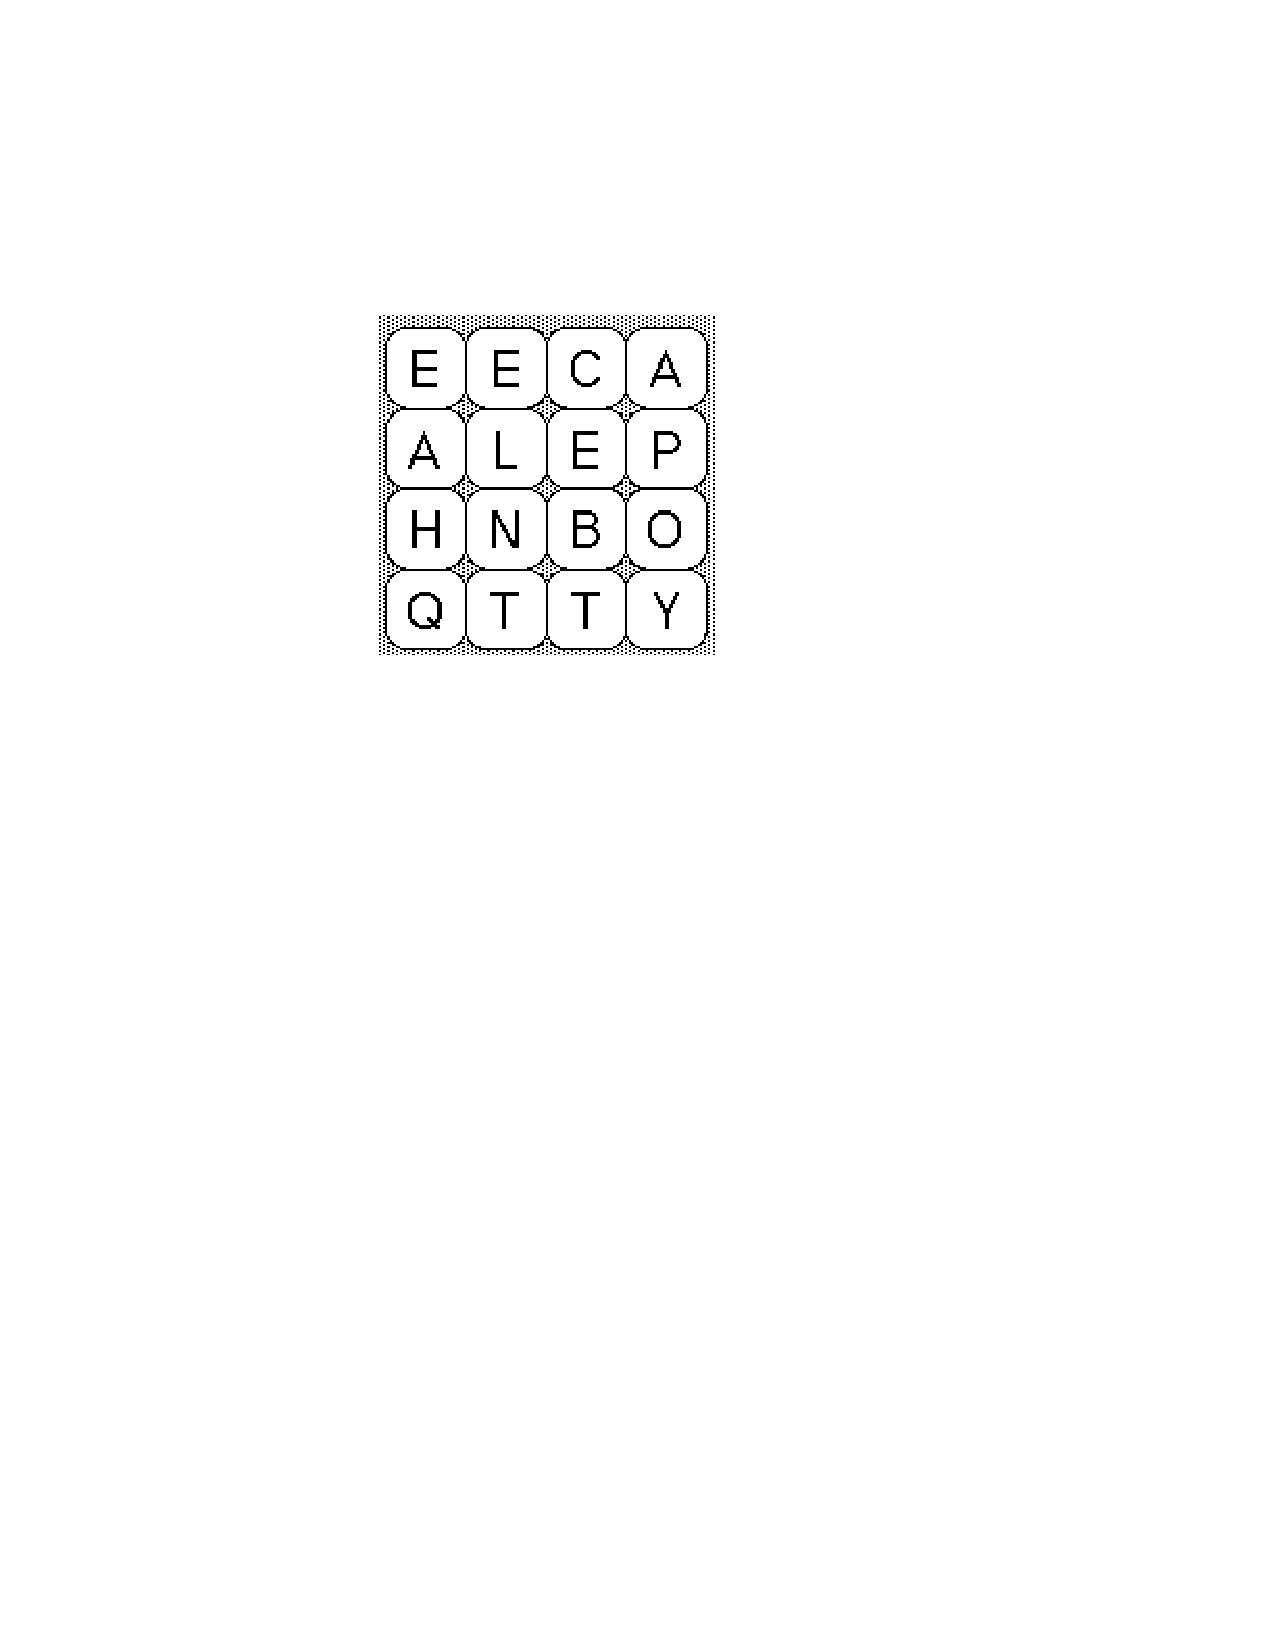
\includegraphics[width=4cm]{grille.pdf}}
\caption{Un exemple de grille. Les mots 'celeb', 'than', 'capo',
  'thane', 'leap' sont présents sur la grille.\label{fig:grille}}
\end{figure}

\section{Implémentation}

On vous demande d'implémenter le jeu tel décrit dans la section précédente.
L'implémentation comprendra 4 parties:

\begin{itemize}
\item \textbf{Chargement du dictionnaire.} Un dictionnaire est utilisé pour
  vérifier que le joueur entre des mots corrects et aussi pour
  guider l'ordinateur lors de sa recherche.
\item \textbf{Tirage et affichage d'une grille.} Vous devez choisir une
  représentation adéquate pour la grille et ajoutez les routines nécessaires
  pour son affichage et sa mise à jour.
\item \textbf{Tour du joueur humain.} Vous devez implémenter la boucle
  permettant au joueur d'entrer ses mots et ensuite les
  différents filtres vérifiant que ces mots sont valides (longueur du
  mot supérieure ou égale à 4, appartenance au dictionnaire, présence
  sur la grille). Dans le cas où le mot est valide, il faut afficher
  la grille où les lettres de ce mot sont mises en évidence et mettre
  à jour le score du joueur.
\item \textbf{Tour de l'ordinateur.} Vous devez implémenter un algorithme
  permettant de retrouver tous les mots du dictionnaire (de 4 lettres
  ou plus) présents sur la grille et ensuite faire l'intersection
  entre cette liste et la liste de mots trouvés par le joueur humain
  pour calculer le score final de l'ordinateur.
\end{itemize}

Nous vous proposons un début d'interface \texttt{Board.h} pour la manipulation
d'une grille et la recherche de mots.  Vous pouvez étendre cette interface avec
les nouvelles fonctions que vous jugerez utiles pour implémenter un jeu complet.
Les fonctions déjà définies dans cette interface doivent être implémentées dans
un fichier \texttt{Board.c} et leurs signatures ne peuvent être modifiées. Vous
êtes par ailleurs libres de modifier \texttt{main.c} et d'ajouter de nouveaux
fichiers si vous jugez cela utile.

Remarques:
\begin{itemize}
\item Dans le fichier \texttt{main.c} que nous vous proposons, le
  dictionnaire est préalablement chargé dans une structure de type
  \texttt{Array}. Pour implémenter la fonction
  \texttt{getAllWordsByBoard} (voir \ref{sec:rechmot}), il est
  cependant nécessaire d'utiliser une structure de données permettant
  de vérifier rapidement l'existence d'un mot dans le dictionnaire,
  par exemple une table de hachage. Vous pouvez créer cette structure
  dans la fonction \texttt{getAllWordsByBoard} à partir de la
  structure de type \texttt{Array}.
\item Le nombre de mots entrés par le joueur, ainsi que le nombre de
  mots trouvés par l'ordinateur sur la grille n'est a priori pas
  connu. Vous devrez donc utiliser une structure de données dynamique
  pour les stocker. Etant donné que ces listes seront relativement
  courtes, vous pouvez utiliser des structures d'accès non efficace
  (type \texttt{Array}).
\item Il ne vous est pas demandé de développer un code générique par
  rapport à la taille de la grille. Vous pouvez donc fixer en dur les
  tailles de vos structures par rapport à la taille de cette dernière.
\item Votre code sera compilé en utilisant la commande:\\
  \texttt{gcc *.c --std=c99 --pedantic -Wall -Wextra -Wmissing-prototypes -o boggle}
\end{itemize}

\section{Algorithmes principaux}

En dehors de la boucle principale du jeu et des interactions avec
le joueur, deux algorithmes non triviaux sont à implémenter:
\begin{itemize}
\item La recherche sur la grille d'un mot entré par l'utilisateur.
\item La recherche de tous les mots du dictionnaire présents sur la
  grille.
\end{itemize}

Nous vous donnons ci-dessous quelques indications sur la manière de
mettre au point ces algorithmes.

\subsection{Recherche d'un mot}

En considérant le grille comme un graphe où chaque n\oe ud correspond
à un dé et chaque arc relie deux dés adjacents, le premier algorithme
s'apparente à un parcours de graphe en profondeur d'abord, parcours
qui devra être initié successivement à partir de tous les n\oe
uds. Nous vous conseillons d'adopter une implémentation récursive. Une
difficulté est d'éviter de passer deux fois par le même n\oe ud lors
de ce parcours et également, contrairement au parcours en profondeur
vu au cours, de bien considérer tous les chemins possibles dans le
graphe (en non pas s'arrêter dès qu'on a visité tous les n\oe
uds). Pour y arriver, vous devrez adopter une stratégie de marquage et
de démarquage des n\oe uds/dés appropriées. Ce marquage pourra se
faire par exemple par le biais d'une structure passée en argument de
la fonction récursive.

Cet algorithme est à implémenter par la fonction \texttt{containsWord}
dans le fichier \texttt{Board.c} et telle que définie dans \texttt{Board.h}.

\subsection{Recherche de tous les mots}\label{sec:rechmot}

On vous demande de comparer trois approches:
\begin{enumerate}
\item Recherche dirigée par la grille (\texttt{getAllWordsByBoard}):
  On parcourt tous les chemins sur la grille et pour chacun d'eux, on
  vérifie si le mot correspondant se trouve dans le
  dictionnaire. Cette approche consiste à modifier l'algorithme de
  recherche d'un mot pour parcourir tous les chemins, et non plus ceux
  qui pourraient correspondre à un mot donné et à stocker au fur et à
  mesure les mots trouvés dans une structure (qui sera par exemple
  ajoutée dans les arguments de la fonction
  récursive). L'implémentation de cette variante ne devrait pas poser
  de problème une fois que vous aurez implémenté la recherche d'un
  mot.
\item Recherche dirigée par le dictionnaire
  (\texttt{getAllWordsByDictionary}): On parcourt les mots du
  dictionnaire et on recherche chacun d'eux séparément sur la grille à
  l'aide de la fonction de recherche d'un mot sur une
  grille. L'implémentation de cette variante est triviale sur base de
  la fonction de recherche d'un mot.
\item Recherche dirigée par le dictionnaire + pré-filtrage
  (\texttt{getAllWordsByDynamicProgramming}): Même approche que
  précédemment mais où avant d'appliquer la recherche par parcours du
  graphe on utilisera une méthode par programmation dynamique efficace
  pour rejeter rapidement certains mots (voir les détails plus bas).
\end{enumerate}

Ces variantes sont à implémenter dans le fichier \texttt{Board.c} et telles que
définies dans \texttt{Board.h}.


\paragraph{Filtrage par programmation dynamique.}

Si on n'impose plus qu'un chemin ne peut pas passer deux fois par le
même dé sur la grille (en maintenant cependant l'obligation de se
déplacer vers un dé adjacent à chaque lettre), il est possible
d'implémenter l'algorithme de recherche d'un mot sur la grille de
manière efficace par programmation dynamique.

Supposons que les positions dans la grille soient numérotées de 1 à
16, de gauche à droite et de {\color{red} haut en bas}, et notons $N$
la taille du mot recherché. La solution par programmation dynamique
consiste à remplir une table $M$ de taille $16\times N$ telle que
$M[i][n]=true$ ($\forall i\in\{1,\ldots,16\}$ et $n\in\{1,\ldots,N\}$)
s'il y a un chemin dans la grille qui s'arrête à la position $i$ et
qui {\color{red} correspond exactement} au préfixe du mot recherché de
taille $n$, $false$ sinon. {\color{red} Exemples:
\begin{itemize}
\item Si on recherche le mot 'celeb' dans la grille de la figure
  \ref{fig:grille}, la valeur de $M[6][3]$ sera $true$ car le chemin
  3-2-6 se terminant à la position 6 correspond au préfixe de taille 3
  du mot 'celeb' (c'est-à-dire 'cel').
\item Si le mot recherché est 'cecity', $M[3][3]$ sera $true$ car le
  chemin 3-7-3 (qui n'est pas un chemin valide selon les règles du
  boggle puisqu'il passe deux fois par la position 3) correspond à
  'cec' qui est le préfixe de taille 3 de 'cecity'.
\end{itemize}}

Un mot sera alors présent sur la grille, au sens relaxé, dès qu'il
existe un $i$ tel que $M[i][N]=true$. Du point de vue de votre
implémentation de cette fonction, il est intéressant de noter que
$M[i][n]=false$ pour tout $i$ implique que
$M[i][n']{\color{red}=false}$ pour tout $i$ et pour tout $n'$ tel
$N\geq n'>n$ (dès qu'un préfixe du mot n'est pas accepté, on sait
qu'il en sera de même pour le mot complet). {\color{red} Il est donc
  inutile de poursuivre le remplissage de la table dès que tous les
  éléments d'une colonne sont $false$.}

Si un mot n'est pas trouvé sur la grille par cet algorithme, il ne
sera évidemment pas non plus trouvé selon les règles
originales. L'idée de la variante que nous demandons d'implémenter
 par la fonction \texttt{getAllWordsByDynamicProgramming} est basée sur les étapes suivantes:
\begin{itemize}
\item Pour tous les mots de plus de 3 lettres dans le dictionnaire:
\begin{itemize}
\item Calculer la table $M$
\item S'il n'existe pas de $i$ tel que $M[i][N]$ est vrai, rejeter le mot.
\item Sinon, rechercher ce mot dans la grille à l'aide de la fonction
  \texttt{containsWord}.
\item Si le mot est trouvé sur la grille, l'ajouter à la liste des mots de l'ordinateur.
\end{itemize}
\end{itemize}
Cette variante devrait améliorer les performances si le calcul de la
table est efficace et s'il y a peu de mots du dictionnaire détectés
sur la grille lorsqu'on permet de passer plusieurs fois par un même
dé.

\section{Questions}

Votre rapport devra contenir les réponses aux questions suivantes:
\begin{enumerate}
\item Décrivez en pseudo-code l'algorithme de recherche d'un mot sur
  une grille.
\item Donnez la formulation récursive permettant de calculer les
  éléments de la table $M$, en précisant bien le ou les cas de
  base. Vous pouvez supposer que vous disposer d'une fonction
  $getNeighbors(i)$ renvoyant la liste des positions adjacentes à la
  position $i$ sur la grille.
\item En déduire le pseudo-code de la fonction de remplissage de la
  table (par l'approche ascendante ou descendante).
\item Donnez la complexité de cet algorithme en fonction de la
  longueur du mot et de la taille de la grille.
\item Mesurez les temps de calcul des trois variantes de l'algorithme
  de recherche de tous les mots sur une grille en faisant une moyenne
  sur 10 grilles générées aléatoirement et commentez ces résultats.
\end{enumerate}

\end{document}
